\subsubsection{Naive Bayes Results}

\begin{table}[H]
\centering
\caption{Classification Report for Naïve Bayes Classifier using TF-IDF features}
\label{tab:nb_classification_report}
\begin{tabular}{lcccc}
\toprule
Class        & Precision & Recall & F1-score & Support \\
\midrule
0            & 0.85      & 0.83   & 0.84     & 4654    \\
1            & 0.84      & 0.86   & 0.85     & 4887    \\
\midrule
Accuracy     &           &        & 0.85     & 9541    \\
Macro Avg    & 0.85      & 0.85   & 0.85     & 9541    \\
Weighted Avg & 0.85      & 0.85   & 0.85     & 9541    \\
\bottomrule
\end{tabular}
\end{table}

\begin{figure}[H]
    \centering
    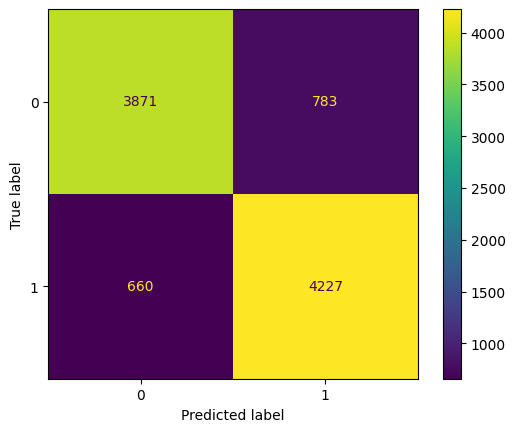
\includegraphics[width=0.45\textwidth]{images/confusion_matrix_nb.png}
    \caption{Confusion matrix for the Naïve Bayes model using TF-IDF features}
    \label{fig:confusion_nb}
\end{figure}

\begin{figure}[H]
    \centering
    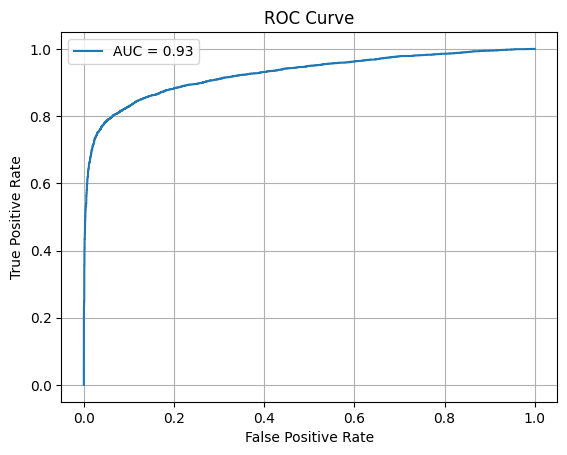
\includegraphics[width=0.45\textwidth]{images/roc_curve_nb.png}
    \caption{ROC curve for the Naïve Bayes classifier with an AUC of 0.93}
    \label{fig:roc_nb}
\end{figure}


The Naïve Bayes classifier achieved competitive results using TF-IDF representations as input features. As shown in Table~\ref{tab:nb_classification_report}, the model attained a balanced performance across both classes, with an F1-score of 0.84 for class 0 (non-hate) and 0.85 for class 1 (hate). The overall accuracy was 85\%, which is comparable to more complex architectures, demonstrating the effectiveness of probabilistic models for text classification tasks with well-engineered features.

The confusion matrix in Figure~\ref{fig:confusion_nb} shows that the classifier correctly predicted 3871 non-hate and 4227 hate speech instances. However, it also misclassified 660 hate comments as non-hate and 783 non-hate comments as hate, indicating a slightly better recall for the hate class.

Furthermore, the ROC curve in Figure~\ref{fig:roc_nb} presents an Area Under the Curve (AUC) of 0.93, which confirms the model’s strong ability to discriminate between classes across different thresholds. This result highlights the classifier's reliability in ranking predictions, making it a viable choice for lightweight and interpretable hate speech detection systems.

Despite its simplicity and the conditional independence assumption, the Naïve Bayes classifier provides robust performance, especially when computational efficiency is prioritized or in ensemble learning contexts.